\begin{tikzpicture}
\begin{axis} [
     title={},
     width=\textwidth,
     height=.2\textheight,
     xlabel={\footnotesize \textbf{Concept}},
     ylabel={\footnotesize \textbf{Frequency}},
     bar width = 4pt,
     ybar = .02cm,
     xmin=0, xmax=7,
     ymin=0.0, ymax=200,
     xtick=data,
     x tick label style={font=\tiny,align=center},
     y tick label style={font=\tiny},
     xtick={1,2,3,4,5,6},
     xticklabels={{Colour \& \\ Appearance}, {Location \& \\ Position}, {Objects \\ Parts}, {Context}, {Objects \&\\Entities}, {State}},
     y label style={at={(axis description cs:0.05,.5)},anchor=south},
     x label style={at={(axis description cs:0.5,-.07)},anchor=north},
     ymajorgrids=false,
     xmajorgrids=false,
     legend style={
			at={(0.5,-0.45)},
			anchor=north,
			legend columns=5,
            }
] 

%{'a': 32, 'b': 21, 'c': 37, 'd': 19, 'e': 144, 'f': 3}
\addplot[color=red, fill=red,  area legend] coordinates {(1, 32) (2, 21) (3, 37) (4, 19) (5, 144) (6, 3)};

%{'a': 35, 'b': 16, 'c': 38, 'd': 17, 'e': 143, 'f': 3}
\addplot[color=red!50, fill=red!50,  area legend] coordinates {(1, 35) (2, 16) (3, 38) (4, 17) (5, 143) (6, 3)};

%{'a': 36, 'b': 15, 'c': 56, 'd': 2, 'e': 114, 'f': 25}
\addplot[color=blue, fill=blue,  area legend] coordinates {(1, 36) (2, 15) (3, 56) (4, 2) (5, 114) (6, 25)};

\legend{\textbf{Llava (7B)}, \textbf{Llava (13B)},\textbf{Cambrian (8B)}}
  
\end{axis}
\end{tikzpicture}